\documentclass[journal,letterpaper]{IEEEtran}
\usepackage[utf8]{inputenc}
\usepackage[spanish]{babel}
\usepackage{amsmath}
\usepackage{graphicx}
\usepackage{booktabs}
\usepackage{hyperref}
\usepackage{microtype}
\usepackage{array}
\usepackage{multirow}
\graphicspath{
    {../../sprint_01/informes/figures/}
    {../../sprint_02/informes/figures/}
    {../../sprint_03/informes/figures/}
    {../../figures/}
}

\begin{document}

\title{Reporte Final Unificado: Segmentación Predictiva de Clientes Premium en Olist}

\author{Marcelo de la Quintana,
        Gaston Nina,
        y~Gerick Toro\\
        \textit{Módulo de Implementación de Soluciones de Inteligencia Artificial}\\
        \textit{Maestría en Inteligencia Artificial y Ciencia de Datos}}

\markboth{REPORTE FINAL UNIFICADO, JUNIO 2026}%
{Proyecto Olist: Clientes Premium}

\maketitle

\begin{abstract}
Este documento integra de forma unificada el desarrollo completo del proyecto de segmentación predictiva de clientes premium sobre Olist. El trabajo parte del perfilado físico y temporal de siete tablas crudas del negocio, evoluciona hacia un pipeline reproducible de construcción de \textit{features}, selección experimental de variables y entrenamiento supervisado, y culmina en un MVP desplegable con dashboard, API, explicabilidad y criterios de gobernanza. La variable objetivo final se definió como pertenencia al segmento premium a partir del percentil 80 del gasto acumulado de pedidos entregados, con umbral fijo de BRL \textbf{197.01} calculado sobre el conjunto de desarrollo. El baseline inicial de regresión logística obtuvo un ROC-AUC de \textbf{0.5355}, evidenciando la llamada Paradoja del Target: en Olist, el valor del cliente está mucho más asociado a compras únicas de alto monto que a alta recurrencia. La incorporación de variables operativas, logísticas, geográficas, de categoría y comportamiento de pago elevó el desempeño a ROC-AUC \textbf{0.7929} y Gini \textbf{0.5858}. Posteriormente, un benchmark de cinco algoritmos y una optimización con Optuna consolidaron a LightGBM como modelo final, con ROC-AUC de validación \textbf{0.8081}, Gini \textbf{0.6162} y umbral operativo de decisión \textbf{0.55}. El MVP funcional demostró integración reproducible sobre un \textit{backtest} formal de agosto de 2018, explicabilidad local y global vía SHAP, y una simulación financiera donde una campaña focalizada pasa de ROI \textbf{-89.57\%} en estrategia masiva a ROI \textbf{+250.40\%}. Finalmente, se establecen criterios de privacidad, monitoreo y reentrenamiento para mantener la utilidad del modelo frente a cambios del mercado.
\end{abstract}

\begin{IEEEkeywords}
Clientes Premium, Olist, Clasificación Supervisada, Pipeline Reproducible, LightGBM, SHAP, ROI, Gobernanza de Modelos.
\end{IEEEkeywords}

\section{Introducción}
\IEEEPARstart{L}{a} identificación temprana de clientes de alto valor es una capacidad crítica para cualquier plataforma de comercio electrónico que busque optimizar campañas de retención, venta cruzada y asignación presupuestaria. En Olist, esta necesidad es especialmente relevante porque una fracción relativamente pequeña de clientes concentra una porción desproporcionada de la facturación. Sin embargo, esa concentración no surge de un patrón clásico de lealtad y recompra frecuente, sino de compras únicas de alto monto, lo que vuelve insuficiente la segmentación tradicional basada únicamente en RFM.

El objetivo general del proyecto fue construir un sistema reproducible para clasificar clientes premium a nivel \texttt{customer\_unique\_id}, partiendo de datos históricos de órdenes, pagos, entregas, reseñas y catálogo. El alcance no se limitó al entrenamiento de un clasificador: también incluyó limpieza y perfilado de calidad de datos, definición formal del target, ingeniería de variables, comparación de algoritmos, construcción de un artefacto serializado y despliegue de un MVP con dashboard, API y criterios de uso responsable.

\section{Datos, Calidad y Comprensión del Problema}
El proyecto se construyó sobre siete datasets crudos de Olist: clientes, órdenes, pagos, reseñas, productos, vendedores e ítems de compra. El perfilado inicial reveló tres hallazgos que condicionaron todo el desarrollo posterior.

Primero, la calidad de los datos no era completamente transparente. Se detectaron nulos lógicos en campos de reseñas y fechas operativas, así como inconsistencias cronológicas en el ciclo de vida de pedidos, por ejemplo registros de entrega al transportista anteriores a la aprobación del pago o incluso a la compra. Estas anomalías confirmaron la necesidad de reglas explícitas de saneamiento antes de modelar.

Segundo, la distribución monetaria presentaba una cola larga extrema. La asimetría del gasto acumulado por cliente alcanzó un valor de \textbf{7.92}, lo que descartó el uso de promedios simples como mecanismo robusto de segmentación y favoreció una definición basada en percentiles.

Tercero, el comportamiento del negocio mostró una estructura muy desbalanceada: el \textbf{97\%} de los clientes tenía solo una orden. Esto anticipó que las variables RFM tradicionales tendrían poder limitado para discriminar clientes premium.

\begin{figure}[h]
  \centering
  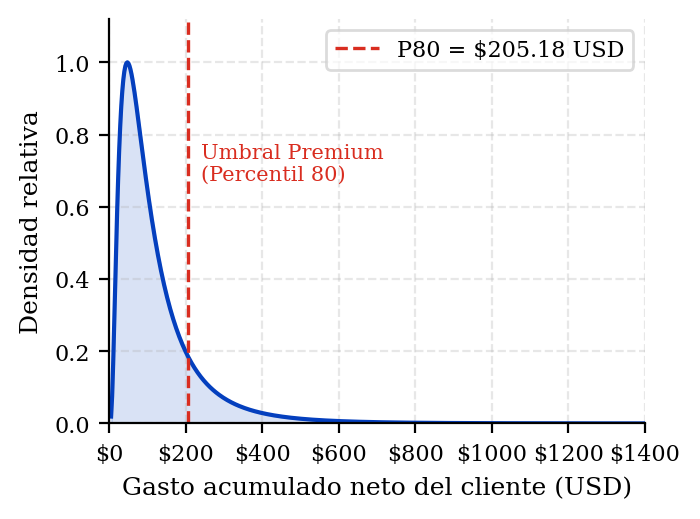
\includegraphics[width=\columnwidth]{fig_long_tail.png}
  \caption{Distribución del gasto acumulado neto por cliente. La cola derecha justifica una segmentación robusta basada en percentiles.}
  \label{fig:long_tail_final}
\end{figure}

\section{Definición del Target y Defensa de Negocio}
La variable objetivo final se definió como:
\begin{equation}
is\_premium =
\begin{cases}
1 & \text{si } total\_spent \geq P80_{dev} = 197.01 \\
0 & \text{en caso contrario}
\end{cases}
\end{equation}

Esta formulación presenta cuatro ventajas metodológicas. Primero, conserva una proporción premium cercana al \textbf{20\%}, interpretable desde negocio como un segmento de alto valor sin volverlo demasiado amplio. Segundo, usa exclusivamente gasto realizado en pedidos \texttt{delivered}, evitando mezclar ingreso concretado con operaciones fallidas. Tercero, congela el umbral sobre el conjunto de desarrollo para mantener comparabilidad entre corridas. Cuarto, permite operar el pipeline en modo \texttt{fit}/\texttt{apply}, separando el cálculo inicial del umbral de sus usos posteriores.

La solidez del target no depende solo de un criterio estadístico. También se valida desde negocio: sobre 96,096 clientes, el segmento premium concentra el \textbf{56.03\%} de la facturación observada y presenta un ticket promedio de BRL \textbf{402.66}, frente a BRL \textbf{92.27} del segmento regular, es decir, un ratio de \textbf{4.36x}. Esto muestra que la etiqueta no está capturando ruido, sino un estrato económicamente relevante.

\begin{table}[h]
\centering
\caption{KPIs de Negocio del Segmento Premium}
\label{tab:kpis_final}
\begin{tabular}{lrr}
\toprule
Indicador & Premium & Regular \\
\midrule
Clientes & 19,220 (20.00\%) & 76,876 (80.00\%) \\
Facturación & BRL 8,088,732 & BRL 6,348,316 \\
Participación facturación & 56.03\% & 43.97\% \\
Ticket promedio & BRL 402.66 & BRL 92.27 \\
\bottomrule
\end{tabular}
\end{table}

\section{Construcción del Pipeline Reproducible}
Una vez defendido el target, el proyecto migró desde notebooks exploratorios hacia un pipeline reproducible en \texttt{src/}. La secuencia operacional quedó estructurada en cuatro pasos:
\begin{enumerate}
    \item construcción de la master table;
    \item generación de variables RFM enriquecidas;
    \item selección experimental de variables;
    \item evaluación supervisada del modelo.
\end{enumerate}

La master table consolidó información a nivel \texttt{customer\_unique\_id}, integrando métricas operativas, financieras, logísticas, geográficas y de catálogo. Tras limpieza, quedó con 96,096 filas, 33 columnas y cero duplicados por identificador. Sobre esta base se construyeron \textbf{18 variables nuevas}, incluyendo indicadores de cuotas, complejidad de pago, retrasos logísticos, agrupación geográfica y categoría principal del cliente.

El control de fuga de información fue una restricción central. Se excluyeron del espacio de modelado las proxies monetarias directas del target, como \texttt{total\_spent}, \texttt{avg\_ticket}, \texttt{avg\_order\_price}, \texttt{avg\_item\_price} y afines. También se eliminaron identificadores y atributos operativos que no debían participar en predicción, como \texttt{customer\_unique\_id}, \texttt{customer\_city}, \texttt{customer\_zip\_code\_prefix}, \texttt{first\_purchase} y \texttt{last\_purchase}.

\section{Selección de Variables y Salto sobre el Baseline}
La primera versión del clasificador fue una regresión logística libre de leakage. Su desempeño fue deliberadamente humilde: \textbf{Precision = 0.30}, \textbf{Recall = 0.16}, \textbf{F1 = 0.21} y \textbf{ROC-AUC = 0.5355}. Este resultado confirmó que la definición del problema era válida, pero también que el set inicial de variables no capturaba adecuadamente el comportamiento premium.

\begin{figure}[h]
  \centering
  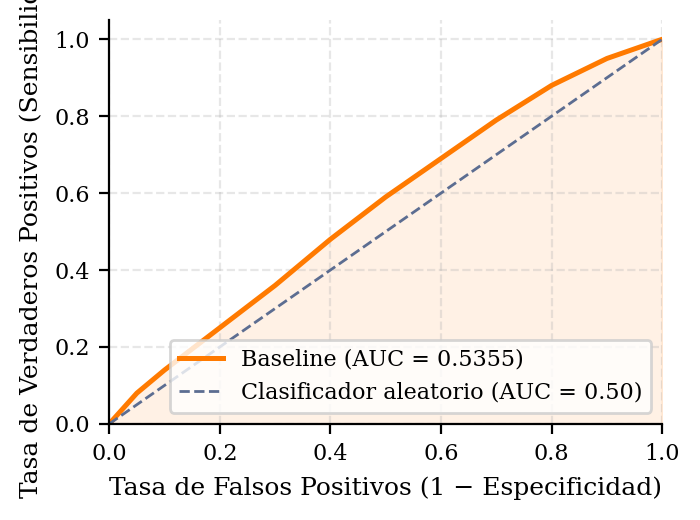
\includegraphics[width=\columnwidth]{fig_roc_baseline.png}
  \caption{Curva ROC del baseline logístico. El rendimiento apenas superior al azar evidenció la insuficiencia del esquema inicial.}
  \label{fig:roc_baseline_final}
\end{figure}

Para resolver esta limitación se ejecutaron \textbf{ocho experimentos reproducibles de selección de variables} con split temporal oficial en \texttt{2018-07-01}. El experimento ganador fue \texttt{corr\_le\_0.85}, que retuvo \textbf{28 variables} con una pérdida despreciable de AUC frente al set inicial, a cambio de menor redundancia y mayor parsimonia.

\begin{figure}[h]
  \centering
  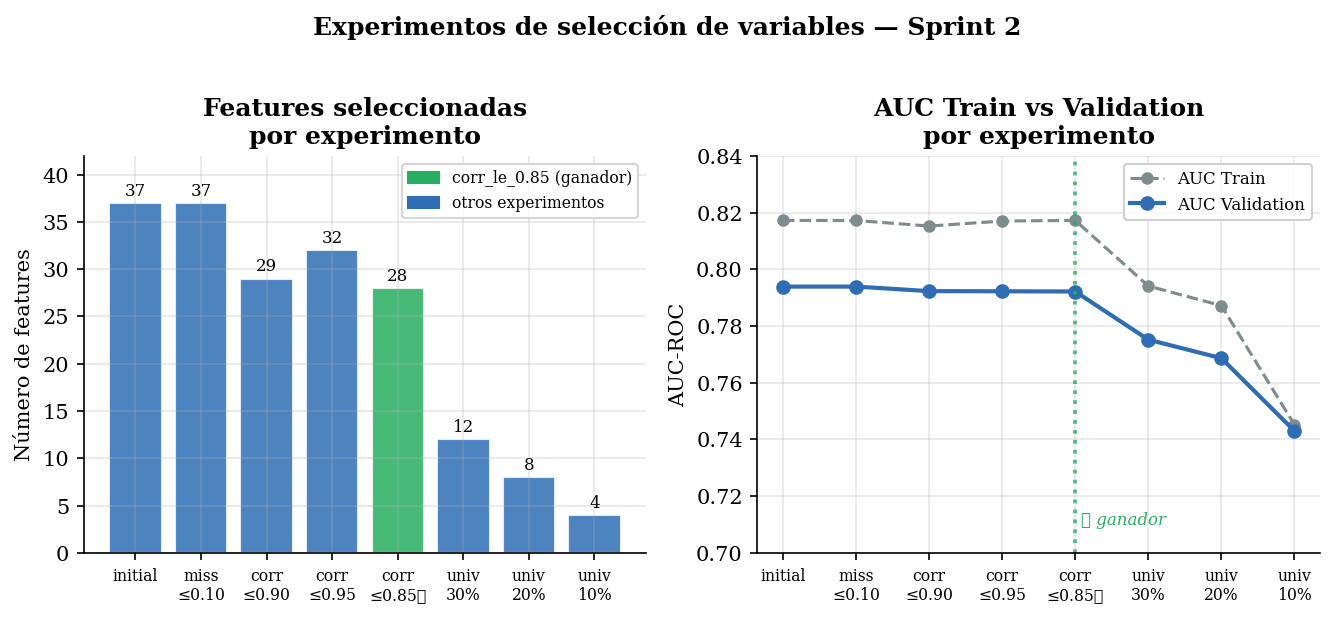
\includegraphics[width=\columnwidth]{fig_feature_selection.png}
  \caption{Comparación de experimentos de selección de variables. El set final balancea desempeño y parsimonia.}
  \label{fig:feature_selection_final}
\end{figure}

Con este set enriquecido, el desempeño mejoró de forma sustancial. El modelo de referencia de esta etapa alcanzó \textbf{Precision = 0.4766}, \textbf{Recall = 0.6294}, \textbf{F1 = 0.5424}, \textbf{ROC-AUC = 0.7929} y \textbf{Gini = 0.5858}. El salto respecto al baseline fue lo suficientemente grande como para afirmar que el problema no era la imposibilidad de predecir el segmento premium, sino la pobreza del espacio inicial de variables.

\begin{table}[h]
\centering
\caption{Evolución de Métricas: Baseline vs. Pipeline Enriquecido}
\label{tab:baseline_vs_pipeline}
\begin{tabular}{lrr}
\toprule
Métrica & Baseline & Pipeline enriquecido \\
\midrule
Precision & 0.3000 & 0.4766 \\
Recall & 0.1600 & 0.6294 \\
F1-Score & 0.2100 & 0.5424 \\
ROC-AUC & 0.5355 & 0.7929 \\
Gini & 0.0710 & 0.5858 \\
\bottomrule
\end{tabular}
\end{table}

\section{Selección del Modelo Final}
Con el set de 28 variables consolidado, se evaluaron cinco algoritmos candidatos: Regresión Logística, Random Forest, Gradient Boosting, XGBoost y LightGBM. El benchmark confirmó que los modelos de boosting ofrecían la mejor combinación entre discriminación global y cobertura del segmento premium.

La selección no se basó únicamente en ROC-AUC. Se utilizó un criterio compuesto que también consideró Gini, F1 y estabilidad de generalización. Esta decisión evitó elegir modelos con AUC competitivo pero Recall insuficiente para negocio.

Los finalistas fueron LightGBM y XGBoost. Luego se ejecutó optimización de hiperparámetros con \textbf{Optuna TPE}, 50 \textit{trials} por modelo. LightGBM emergió como ganador con \textbf{ROC-AUC = 0.8081}, \textbf{Gini = 0.6162} y gap de sobreajuste controlado. El umbral operativo seleccionado fue \textbf{0.55}, valor que maximiza el F1-Score.

\begin{figure}[h]
  \centering
  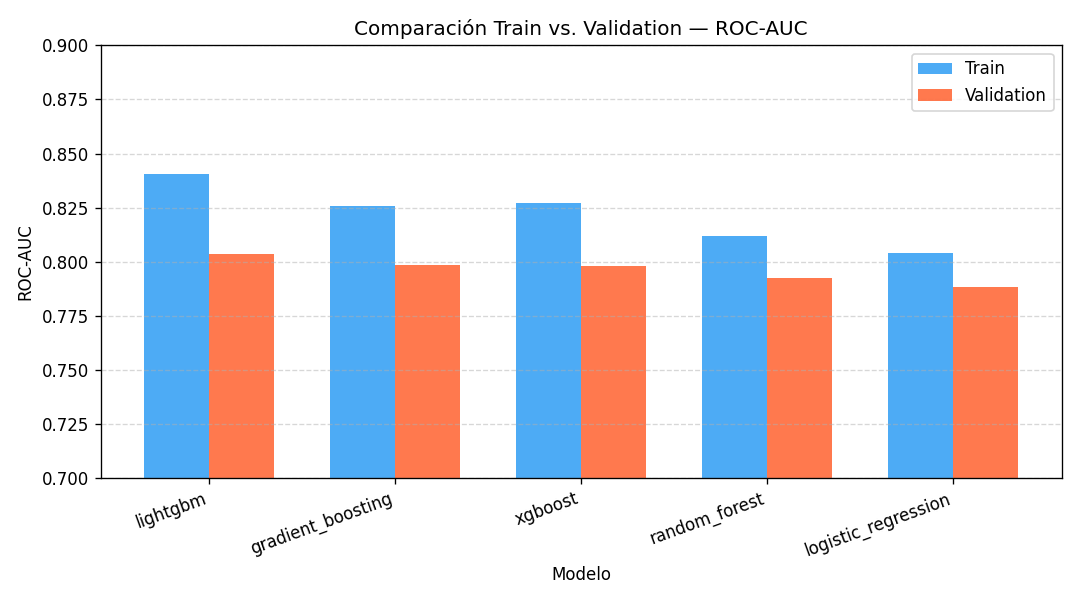
\includegraphics[width=\columnwidth]{fig_benchmark_auc.png}
  \caption{Comparación de ROC-AUC train y validación para los modelos candidatos. LightGBM y XGBoost lideran el benchmark.}
  \label{fig:benchmark_final}
\end{figure}

Las variables más influyentes del modelo final combinaron información de categoría, temporalidad, comportamiento de compra y señales de financiamiento. En la etapa de modelado se observó que \texttt{top\_category} y \texttt{recency\_days} concentraban buena parte de la ganancia del clasificador, reforzando que el contexto del producto y la cercanía temporal de la compra son mejores discriminadores que la simple frecuencia.

\section{Despliegue del MVP y Validación Operativa}
El artefacto final se serializó como \texttt{modelo\_final.pkl} y se integró dentro de un MVP compuesto por dos superficies: un dashboard en Streamlit y una API mínima en FastAPI. Ambas consumen el mismo pipeline serializado y comparten el mismo esquema de features, lo que garantiza consistencia entre scoring visual y scoring programático.

\begin{figure}[h]
  \centering
  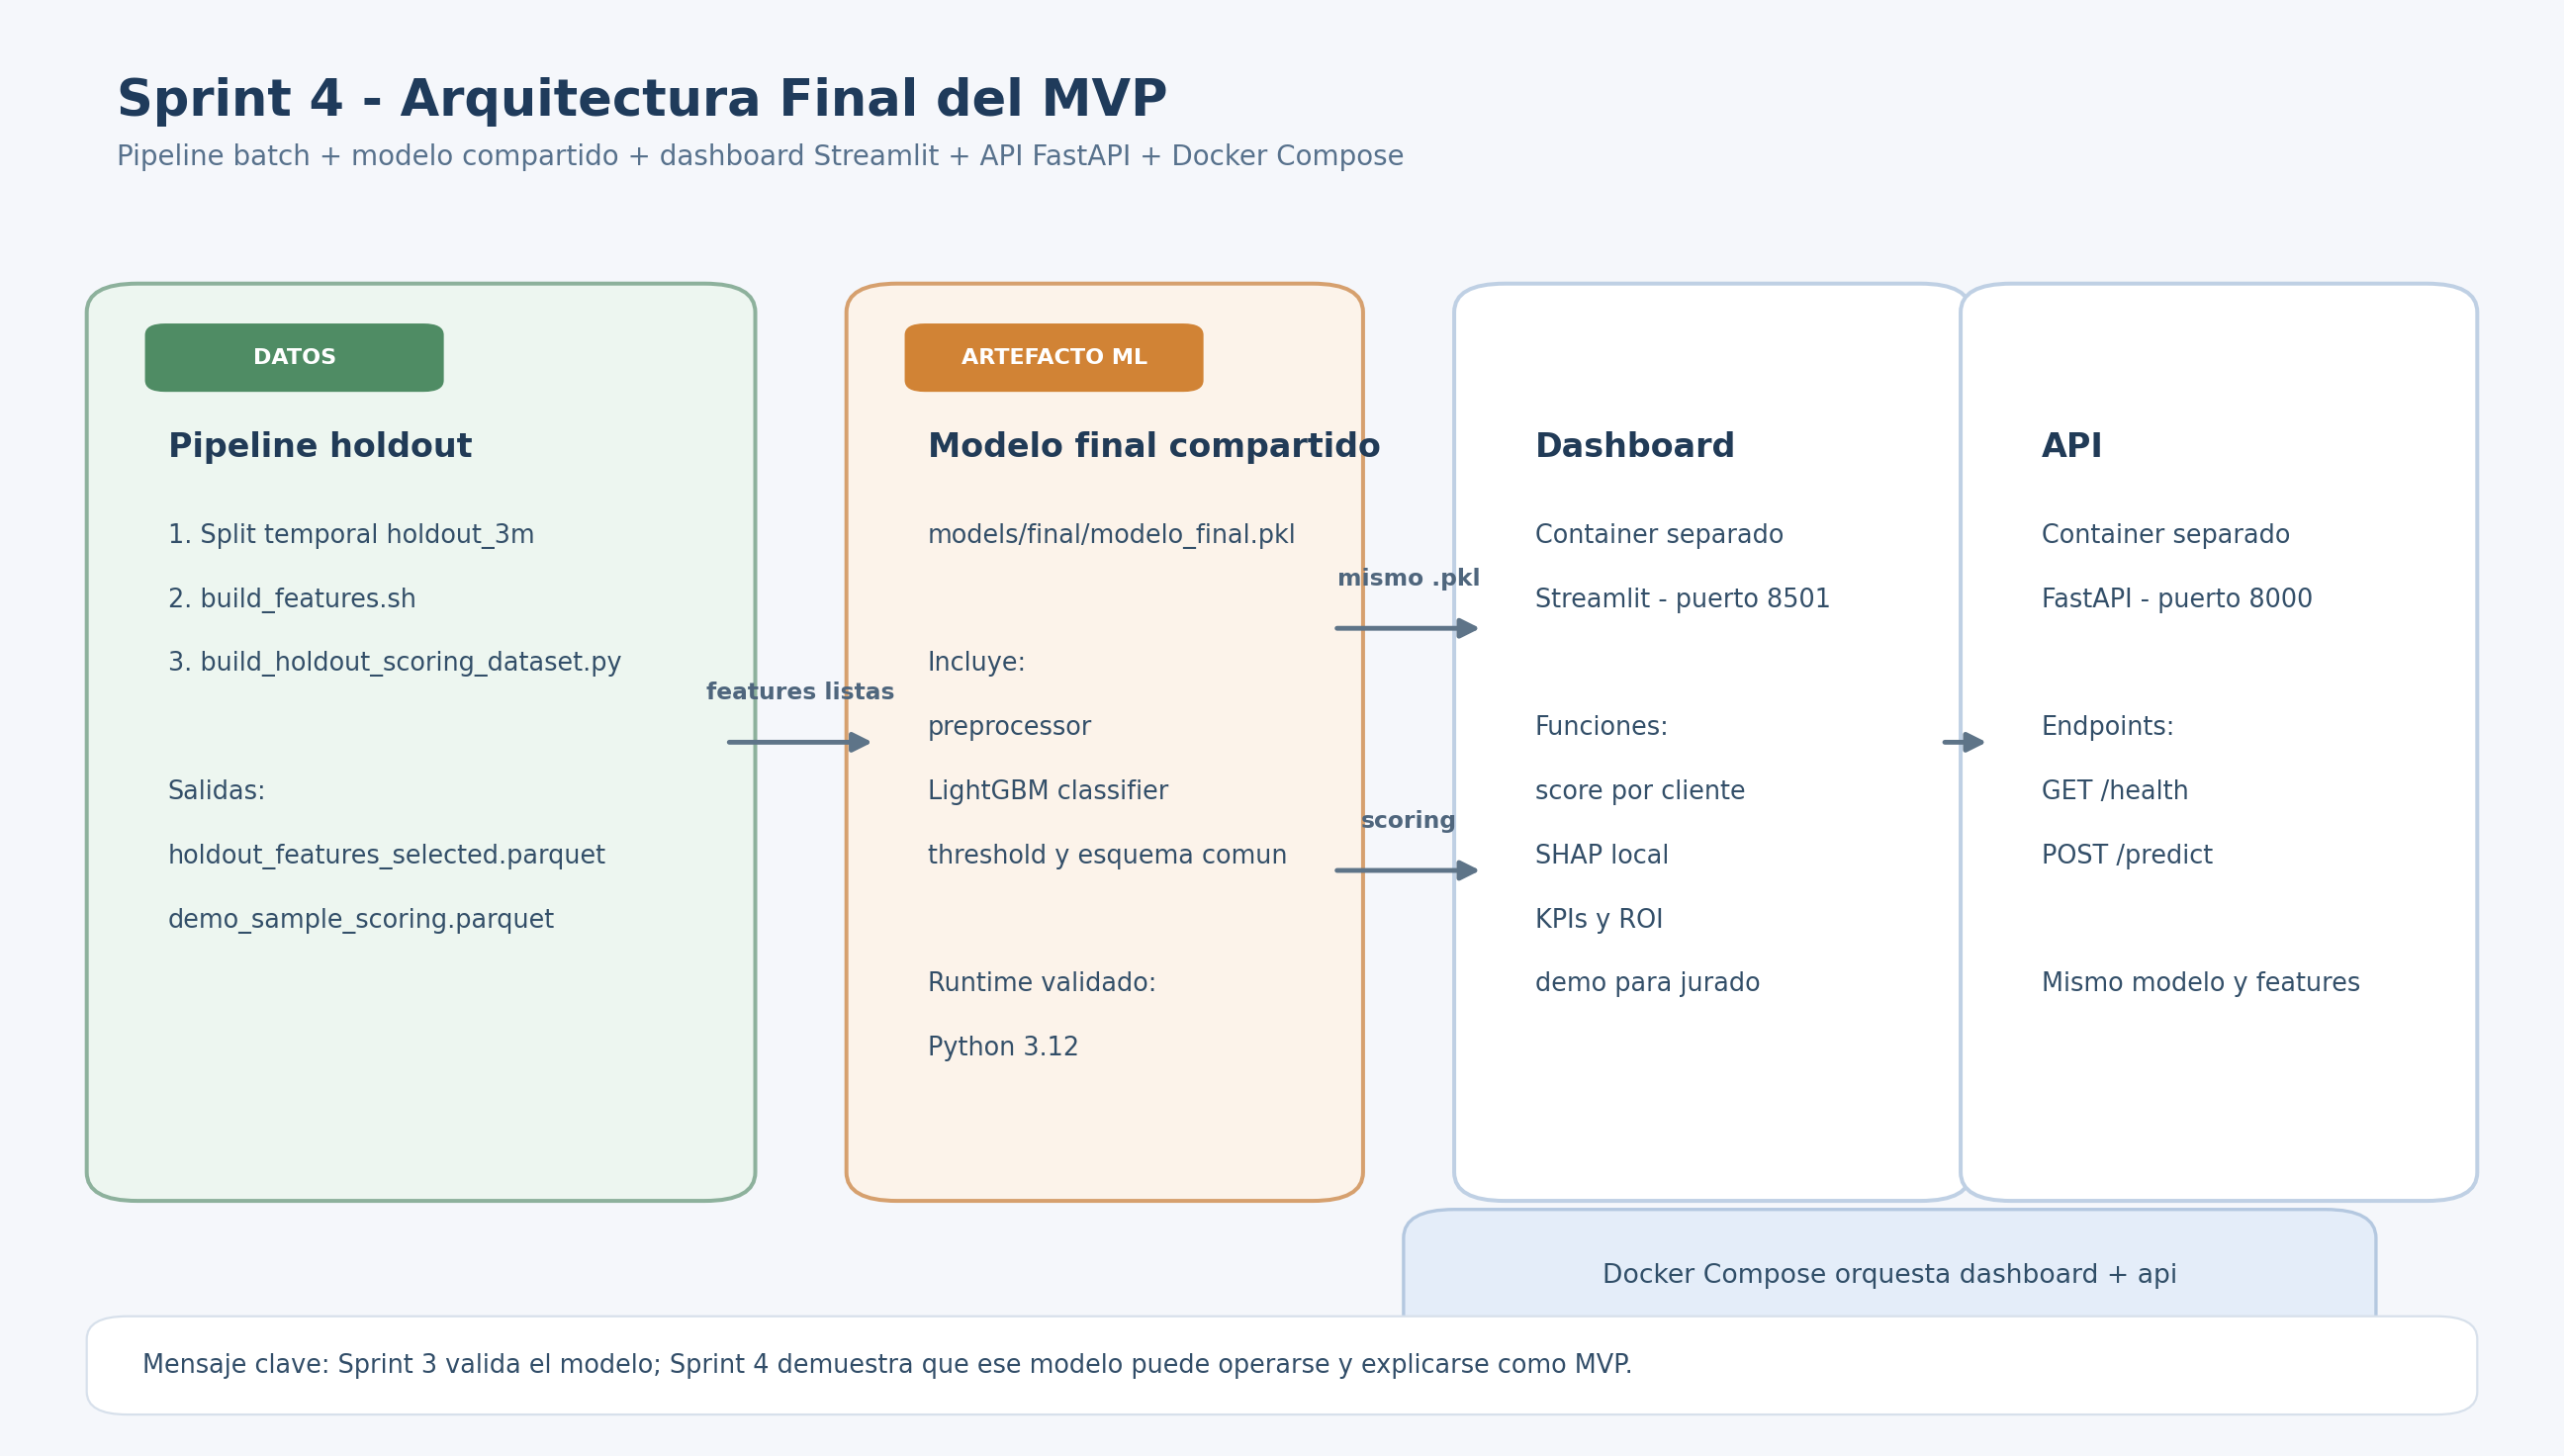
\includegraphics[width=\columnwidth]{sprint_04_mvp_architecture.png}
  \caption{Arquitectura del MVP final. El pipeline genera el dataset de scoring y tanto dashboard como API consumen el mismo modelo serializado.}
  \label{fig:mvp_architecture_final}
\end{figure}

La validación operativa se realizó sobre un \textit{backtest} formal de \textbf{agosto de 2018}. El split técnico histórico \texttt{holdout\_3m} se conservó por trazabilidad, pero septiembre y octubre apenas aportan 20 órdenes combinadas, por lo que no son una base seria para evaluación final. Sobre el \textit{backtest} se obtuvo \textbf{ROC-AUC = 0.9876}, \textbf{Gini = 0.9751}, \textbf{Precision = 43.80\%}, \textbf{Recall = 56.11\%} y \textbf{F1 = 49.20\%}. Este resultado debe leerse con cuidado: no prueba por sí solo una mejora definitiva de generalización, porque agosto de 2018 es estructuralmente más separable y está fuertemente acoplado a la definición del target. La comparación metodológicamente principal sigue siendo la validación temporal del modelo final.

Aun con esa precaución, el \textit{backtest} sí cumple su propósito como prueba de integración: el modelo carga correctamente, produce scoring reproducible, mantiene coherencia con el target congelado y permite construir capas de explicación y simulación económica sobre el mismo artefacto.

Como complemento de negocio, se evaluó el ranking del score mediante una tabla de \textit{lift/gain} en 10 deciles sobre los \textbf{clientes activos en agosto de 2018}. En esta población, la tasa base premium sube a \textbf{19.40\%} y el \textbf{primer decil} captura \textbf{32.32\%} de los premium reales, con una tasa premium interna de \textbf{62.69\%} y un \textbf{lift de 3.23x}. La lectura es más útil comercialmente: el score no ordena una base trivial, sino que concentra valor dentro de la población realmente operativa del backtest.

\section{Explicabilidad e Impacto de Negocio}
El MVP incorporó explicabilidad local mediante \texttt{pred\_contrib=True} de LightGBM y explicabilidad global con un SHAP Summary Plot tipo beeswarm. Las variables dominantes en la explicación global fueron \texttt{delivered\_orders}, \texttt{max\_payment\_installments}, \texttt{total\_items} y \texttt{top\_category\_is\_high\_value}. Esto muestra que el modelo no opera como caja negra arbitraria, sino como una combinación interpretable de intensidad transaccional, valor de categoría y señales de pago.

\begin{figure}[h]
  \centering
  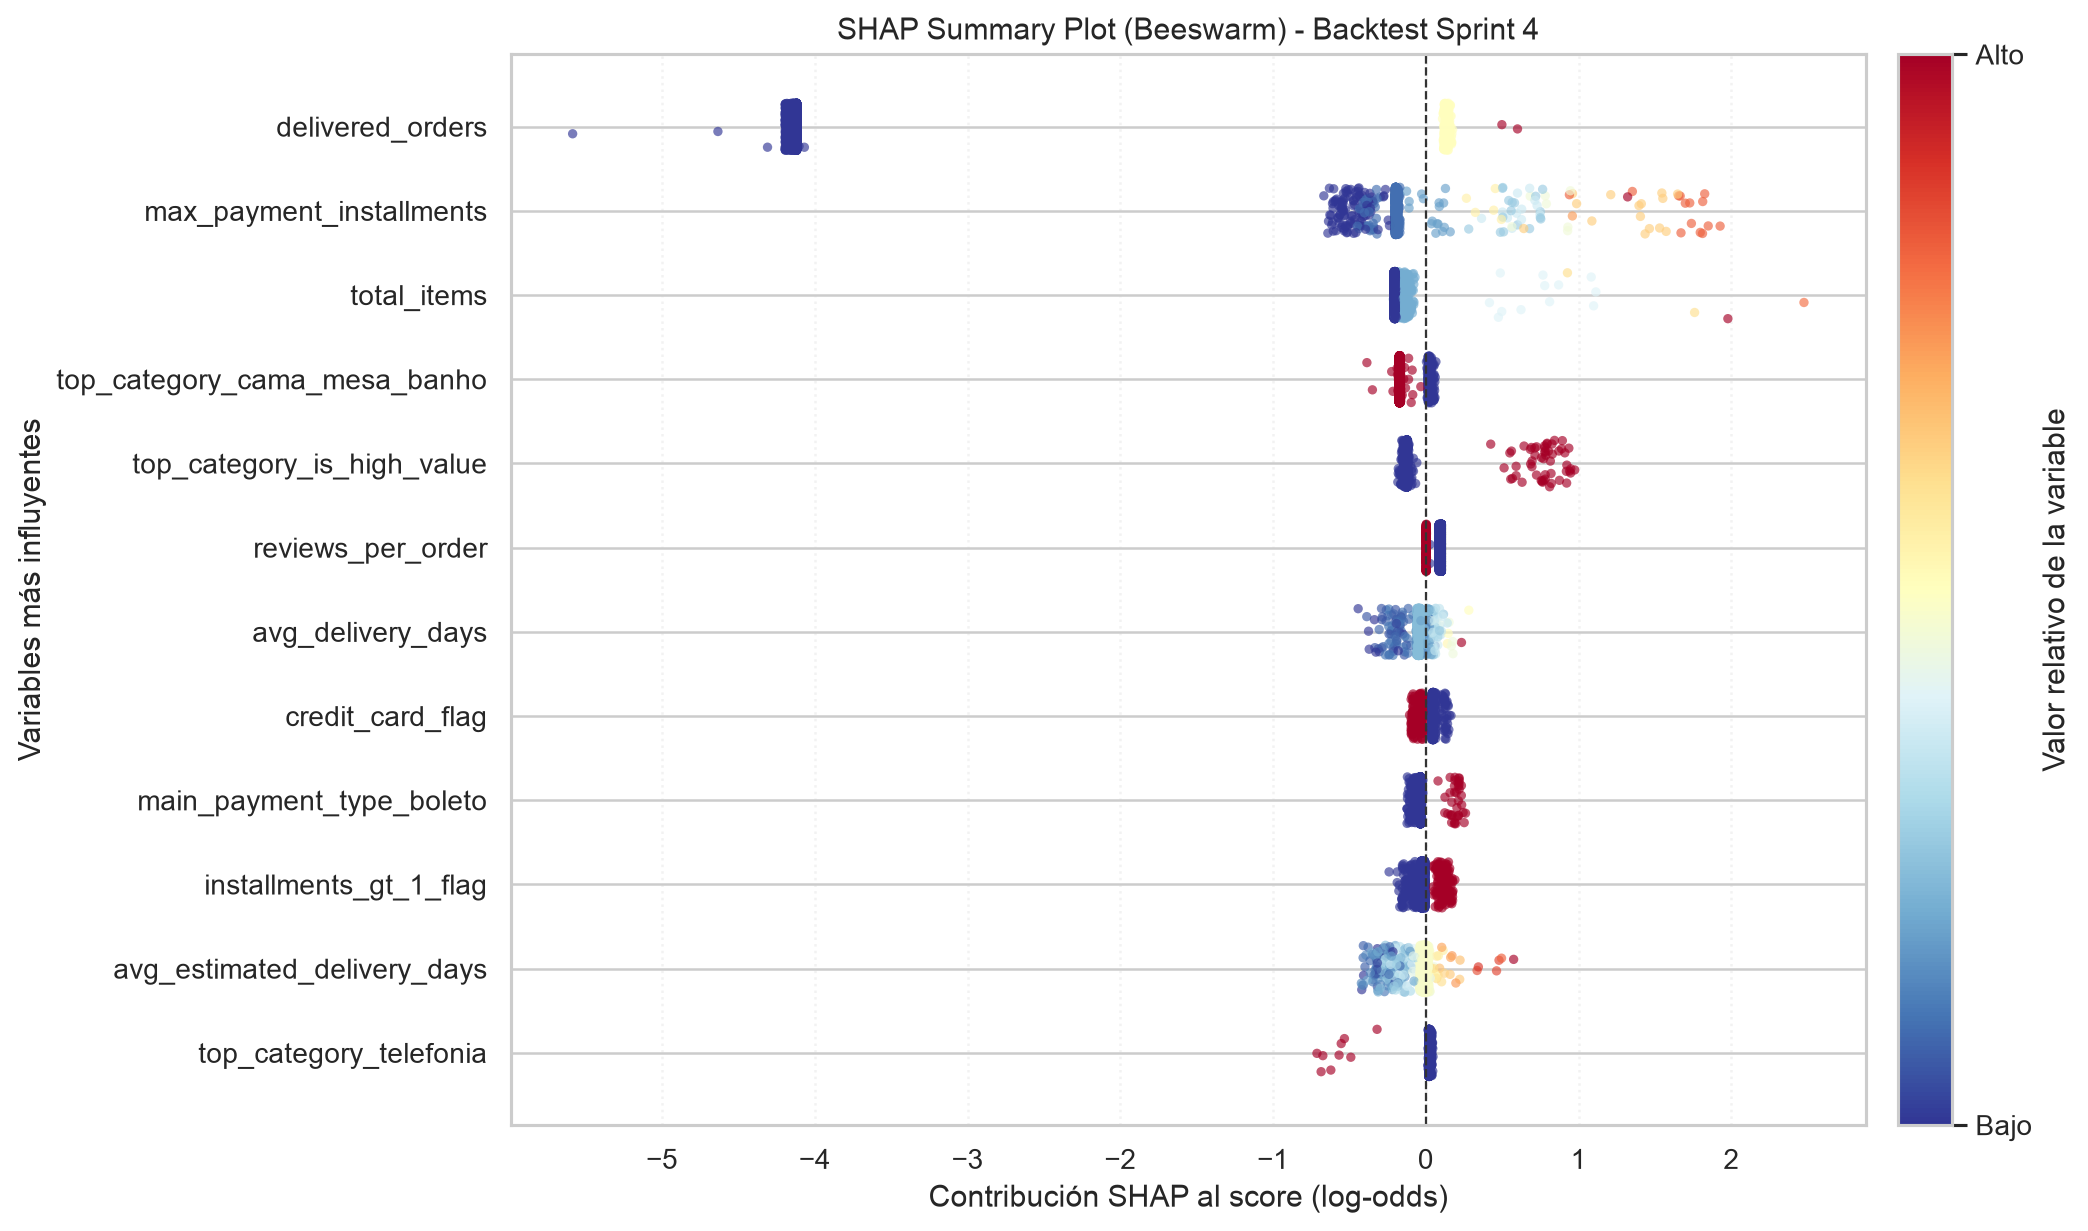
\includegraphics[width=\columnwidth]{sprint_04_shap_beeswarm.png}
  \caption{Explicabilidad global del modelo final sobre una muestra del backtest.}
  \label{fig:shap_final}
\end{figure}

En términos comerciales, se compararon dos estrategias: campaña masiva y campaña focalizada usando el score del modelo. La estrategia masiva implicaría contactar 96,096 clientes, con costo de BRL 1,441,440 y ROI de \textbf{-89.57\%}. En cambio, la campaña focalizada contacta solo 1,605 clientes, reduce drásticamente el costo a BRL 24,075 y alcanza un ROI de \textbf{+250.40\%}. La utilidad neta pasa de una pérdida de BRL 1,291,080 a una ganancia de BRL 60,285.

\begin{table}[h]
\centering
\caption{Comparativa Financiera de Estrategias Comerciales}
\label{tab:roi_final}
\resizebox{\columnwidth}{!}{%
\begin{tabular}{lrr}
\toprule
Métrica & Campaña masiva & Campaña focalizada \\
\midrule
Clientes contactados & 96,096 & 1,605 \\
Costo de campaña & BRL 1,441,440.00 & BRL 24,075.00 \\
Ingreso por conversiones & BRL 150,360.00 & BRL 84,360.00 \\
Utilidad neta & BRL -1,291,080.00 & BRL 60,285.00 \\
ROI & -89.57\% & +250.40\% \\
\bottomrule
\end{tabular}%
}
\end{table}

\section{Privacidad, Gobernanza y Monitoreo}
El proyecto también fue evaluado desde una perspectiva de uso responsable. El modelo final no entrena con datos personales directos ni con identificadores operativos como \texttt{customer\_unique\_id}, \texttt{customer\_city} o \texttt{customer\_zip\_code\_prefix}. Tampoco utiliza datos financieros sensibles directos como números de tarjeta o cuentas bancarias. Sin embargo, sí retiene variables que pueden actuar como proxies de desigualdad, por ejemplo \texttt{customer\_state}, \texttt{main\_payment\_type} o \texttt{max\_payment\_installments}, lo que obliga a mantener supervisión humana y monitoreo de sesgo.

En un contexto operativo, el modelo no debe considerarse vigente para siempre. Se propone monitorear cuatro grupos de señales: desempeño discriminativo, impacto comercial, estabilidad poblacional y drift de variables clave. El criterio recomendado no es reentrenar por calendario fijo, sino por evidencia. Como regla inicial, una caída de Gini superior al 20\% respecto al baseline o un deterioro conjunto de Gini, ROI y tasa premium predicha debería disparar alertas y revisión del artefacto.

Si se confirma degradación, el reentrenamiento debe basarse en una ventana temporal nueva y completa, no en recombinar meses ya vistos por el modelo. Esta distinción evita confundir backtesting histórico con adaptación real a cambios del mercado.

\section{Conclusiones}
El proyecto demostró que la segmentación predictiva de clientes premium en Olist es viable cuando se aborda como un problema integral de datos, modelado y producto, y no solo como ajuste de un clasificador.

Los principales aportes consolidados fueron:
\begin{enumerate}
    \item una definición robusta y defendible del target premium, validada tanto estadística como económicamente;
    \item un pipeline reproducible que transforma datos crudos en un dataset consistente de entrenamiento y scoring;
    \item un salto material de desempeño desde un baseline casi aleatorio hasta un modelo final competitivo y serializable;
    \item un MVP funcional que conecta analítica, scoring, explicabilidad y simulación de negocio;
    \item un marco inicial de privacidad, gobernanza y monitoreo para sostener el uso responsable del modelo.
\end{enumerate}

La principal limitación metodológica es que la validación \textit{backtest} del MVP no debe interpretarse como prueba aislada de superioridad definitiva, dado que la ventana evaluada es más separable que el escenario de validación principal. Aun así, el proyecto cierra con una solución técnicamente sólida, operativamente demostrable y suficientemente defendible para una implementación posterior con monitoreo continuo.

\begin{thebibliography}{3}

\bibitem{rfmt_methodology}
A. Ullah, M. I. Mohmand, H. Hussain, S. Johar, I. Khan, S. Ahmad, H. A. Mahmoud, and S. Huda,
``Customer Analysis Using Machine Learning-Based Classification Algorithms for Effective Segmentation Using Recency, Frequency, Monetary, and Time,''
\emph{Sensors}, vol. 23, no. 6, p. 3180, 2023.

\bibitem{optuna2019}
T. Akiba, S. Sano, T. Yanase, T. Ohta, and M. Koyama,
``Optuna: A Next-generation Hyperparameter Optimization Framework,''
in \emph{Proceedings of the 25th ACM SIGKDD International Conference on Knowledge Discovery \& Data Mining}, 2019.

\bibitem{lightgbm2017}
G. Ke, Q. Meng, T. Finley, T. Wang, W. Chen, W. Ma, Q. Ye, and T.-Y. Liu,
``LightGBM: A Highly Efficient Gradient Boosting Decision Tree,''
in \emph{Advances in Neural Information Processing Systems}, vol. 30, 2017.

\end{thebibliography}

\end{document}
